In this section, we develop the firm's problem under the settings of our DCDP model in continuous time. Following \cite{Estimation-of-Dynamic-Discrete-Choice-Models-in-Continuous-Time_ABBE_2016}, we formulate the value function for a particular potential well site owned by the firm $i$ that is forward-looking and discounts future payoffs at rate $\rho \in (0, \infty)$. Specifically, when the site is in state $k$, its value function is given as follows\footnote{Detailed derivation is presented in \ref{C3-Appendix_Derivations_Value-Function-in-Continuous-Time}.}:
\begin{equation}
\begin{split}
    % \left( \rho \ + \ \sum_{\ell \neq k} \lambda_{k\ell} \ + \ \lambda_{d} \right) V_{ik} \ 
    % & = \ f_{ik} \ + \ \sum_{\ell \neq k} \lambda_{k\ell} V_{i\ell} \ + \ \lambda_{d} E\bigg[ \underset{a}{\max} \left\{ V_{i,\ell(i, a, k)} \ + \ \psi_{iak} \ + \ \epsilon_{iak} \right\} \bigg].
    V_{ik} \ 
    & = 
    \ \frac{
        \ f_{ik} \ + \ \sum_{\ell \neq k} \lambda_{k\ell} V_{i\ell} \ + \ \lambda_{a} E\Big[ \underset{a \in \mathcal{A}}{\max} \left\{ V_{i,\ell(i, a, k)} \ + \ \psi_{iak} \ + \ \epsilon_{iak} \right\} \Big] \ 
    }{
        \rho \ + \ \sum_{\ell \neq k} \lambda_{k\ell} \ + \ \lambda_{a}
    }.
\end{split}
\label{Equation:Firms-Problem_Value-Function}
\end{equation}
For the site, the value function $V_{ik}$ represents the present discounted value of all payoffs obtained from starting at state $k$ and behaving optimally in all subsequent periods.\footnote{Although $V_{ik}$ varies over time, we omit the $t$ subscript for simplicity.} Here, it is assumed that the firm $i$'s drilling decisions have no impact on the price of oil in the market.\footnote{In other words, the assumption implies that the resulting state of taking action $a$ by the firm $i$, denoted $\ell(i, a, k)$, is $k$.} $\dot{V}_{ik}$ is the time derivative of $V_{ik}$. The three terms in the round bracket on the left-hand side are the sum of the discount factor and the rates at which the state can change. The right-hand side consists of the flow payoff, the expected value relying on the firm's decisions, and the rate-weighted value related to exogenous state transitions. The expectation is for the joint distribution of $\epsilon_{i0k}$ and $\epsilon_{i1k}$. While adding in the T1EV cost shocks is tedious, it also allows us to reconcile an empirical, firm-level model with aggregate time paths of resource extraction. 

For a given opportunity to choose an action $a \in \mathcal{A}$, the probability of drilling a horizontal well into the potential site conditional on state $k$, denoted $Pr_{k}$, can be defined as follows\footnote{For given values of parameters, we can compute the value of each $Pr_{k}$, $k = 1, 2, \cdots, K$, by using value function iterations.}:
\begin{equation}
\begin{split}
	Pr_{k} \
	& \equiv \ \Pr \big[ \ \psi_{i1k} + \epsilon_{i1k} \ \geq \ V_{i,\ell(i,0,k)} + \psi_{i0k} + \epsilon_{i0k} \ | \ k \ \big].
\end{split}
\label{Equation:Firms-Problem_CCP}
\end{equation}
As shown in \cite{Estimation-of-Dynamic-Discrete-Choice-Models-in-Continuous-Time_ABBE_2016}, for each action $a \in \mathcal{A}$, the second term on the right-hand side of equation (\ref{Equation:Firms-Problem_Value-Function}) is
\begin{equation}
\begin{split}
	& E\Big[ \underset{a \in \mathcal{A}}{\max} \left\{ V_{i,\ell(i, a, k)} \ + \ \psi_{iak} \ + \ \tilde{\psi}_{iak} \ + \ \epsilon_{iak} \right\} \Big] \\
	& = \ 
	\begin{cases}
		V_{ik} \ + \ \sigma \big( \gamma \ - \ \ln(1 - Pr_{k}) \big) \hspace{1.6cm} \text{if \ \ $a = 0$} \\
		\psi_{i1k} \ + \ \tilde{\psi}_{i1k} \ + \ \sigma \big( \gamma \ - \ \ln(Pr_{k}) \big) \hspace{0.7cm} \text{if \ \ $a = 1$}.
	\end{cases}
\end{split}
\label{Equation:Firms-Problem_Emax}
\end{equation}
where the choice-specific instantaneous payoff function for $a = 1$ (i.e., $\psi_{i1k}$) is the function (\ref{Equation:DCDP-Model_Payoff-Function_Firms-Problem}).

Under the assumption that there is no exogenous demand shock, some algebraic manipulation on the value function (\ref{Equation:Firms-Problem_Value-Function}), with the expressions in (\ref{Equation:Firms-Problem_Emax}), yields the Euler equation that drives the dynamics of the firm's optimal drilling decisions\footnote{See \ref{C3-Appendix_Derivations_Euler-Equation-for-the-Firms-Problem} for details.}:
\begin{equation}
\begin{split}
    % (\rho \ + \ \lambda_{a}) V_{ik} \
    % & = \ f_{ik} \ + \ \lambda_{a} \left\{ \psi_{i1k} \ + \ \sigma \big( \gamma \ - \ \ln(Pr_{k}) \big) \right\} \\
    % (\rho \ + \ \lambda_{a}) \cdot \frac{1}{\rho} \left\{ f_{ik} \ + \ \lambda_{a} \sigma \big( \gamma \ - \ \ln(1 - Pr_{k}) \big) \right\} \
    % & = \ f_{ik} \ + \ \lambda_{a} \left\{ \psi_{i1k} \ + \ \sigma \big( \gamma \ - \ \ln(Pr_{k}) \big) \right\} \\
    % (\rho \ + \ \lambda_{a}) \left\{ f_{ik} \ + \ \lambda_{a} \sigma \big( \gamma \ - \ \ln(1 - Pr_{k}) \big) \right\} \
    % & = \ \rho f_{ik} \ + \ \rho \lambda_{a} \left\{ \psi_{i1k} \ + \ \sigma \big( \gamma \ - \ \ln(Pr_{k}) \big) \right\} \\
    % \lambda_{a} f_{ik} \ + \ (\rho \ + \ \lambda_{a}) \lambda_{a} \sigma \big( \gamma \ - \ \ln(1 - Pr_{k}) \big) \
    % & = \ \rho \lambda_{a} \left\{ \psi_{i1k} \ + \ \sigma \big( \gamma \ - \ \ln(Pr_{k}) \big) \right\} \\
    % f_{ik} \ + \ (\rho \ + \ \lambda_{a}) \sigma \big( \gamma \ - \ \ln(1 - Pr_{k}) \big) \
    % & = \ \rho \left\{ \psi_{i1k} \ + \ \sigma \big( \gamma \ - \ \ln(Pr_{k}) \big) \right\} \\
    % f_{ik} \ + \ \lambda_{a} \sigma \big( \gamma \ - \ \ln(1 - Pr_{k}) \big) \
    % & = \ \rho \left\{ \psi_{i1k} \ + \ \sigma \big( \gamma \ - \ \ln(Pr_{k}) \big) \ - \ \sigma \big( \gamma \ - \ \ln(1 - Pr_{k}) \big) \right\} \\
    \frac{ \ f_{ik} \ + \ \lambda_{a} \sigma \big( \gamma \ - \ \ln(1 - Pr_{k}) \big) \ }{\rho} \
    & = \ \left\{ \psi_{i1k} \ + \ \sigma \big( \gamma \ - \ \ln(Pr_{k}) \big) \right\} \ - \ \sigma \big( \gamma \ - \ \ln(1 - Pr_{k}) \big).
\end{split}
\label{Equation:Firms-Problem_Euler-Equation}
\end{equation}
The left-hand side of this equation represents the sum of the instantaneous change in $V_{ik}$ and the firm's expected payoff when deciding not to drill a horizontal well into the site as the current value at the time point of decision. In the equation, the right-hand side, which is equal to $V_{ik}$ as shown in \ref{C3-Appendix_Derivations_Euler-Equation-for-the-Firms-Problem}, is the firm's payoff if it chooses to drill a horizontal well into the site, including the opportunity cost of the decision. In other words, $V_{ik}$ is the well location's net shadow value as the current value, which is represented as $\pi_{t}$ in the necessary conditions for the social planner's problem. Based on the relationship between $V_{ik}$ and $\pi_{t}$, it is evident that the Euler equation (\ref{Equation:Firms-Problem_Euler-Equation}) drawn from the firm $i$'s well-site-level decisions coincides with the Euler equation (\ref{Equation:Social-Planners-Problem_Euler-Equation}) of the social planner's welfare maximization problem.\footnote{There are two differences between the Euler equations. First, the rate of interest $r$ is used in the social planner's problem, whereas the discount rate $\rho$ is utilized in the firm's problem. Second, we exploit two different choice-specific instantaneous payoff functions, which are demonstrated in (\ref{Equation:DCDP-Model_Payoff-Function_Social-Planners-Problem}) and (\ref{Equation:DCDP-Model_Payoff-Function_Firms-Problem}), in the two dynamic optimization problems. Of note, both of the choice-specific instantaneous payoff functions indicate the net benefit obtained from the output of drilling activities.}
\afterpage{
    \begin{figure}[t!]
        \centering
        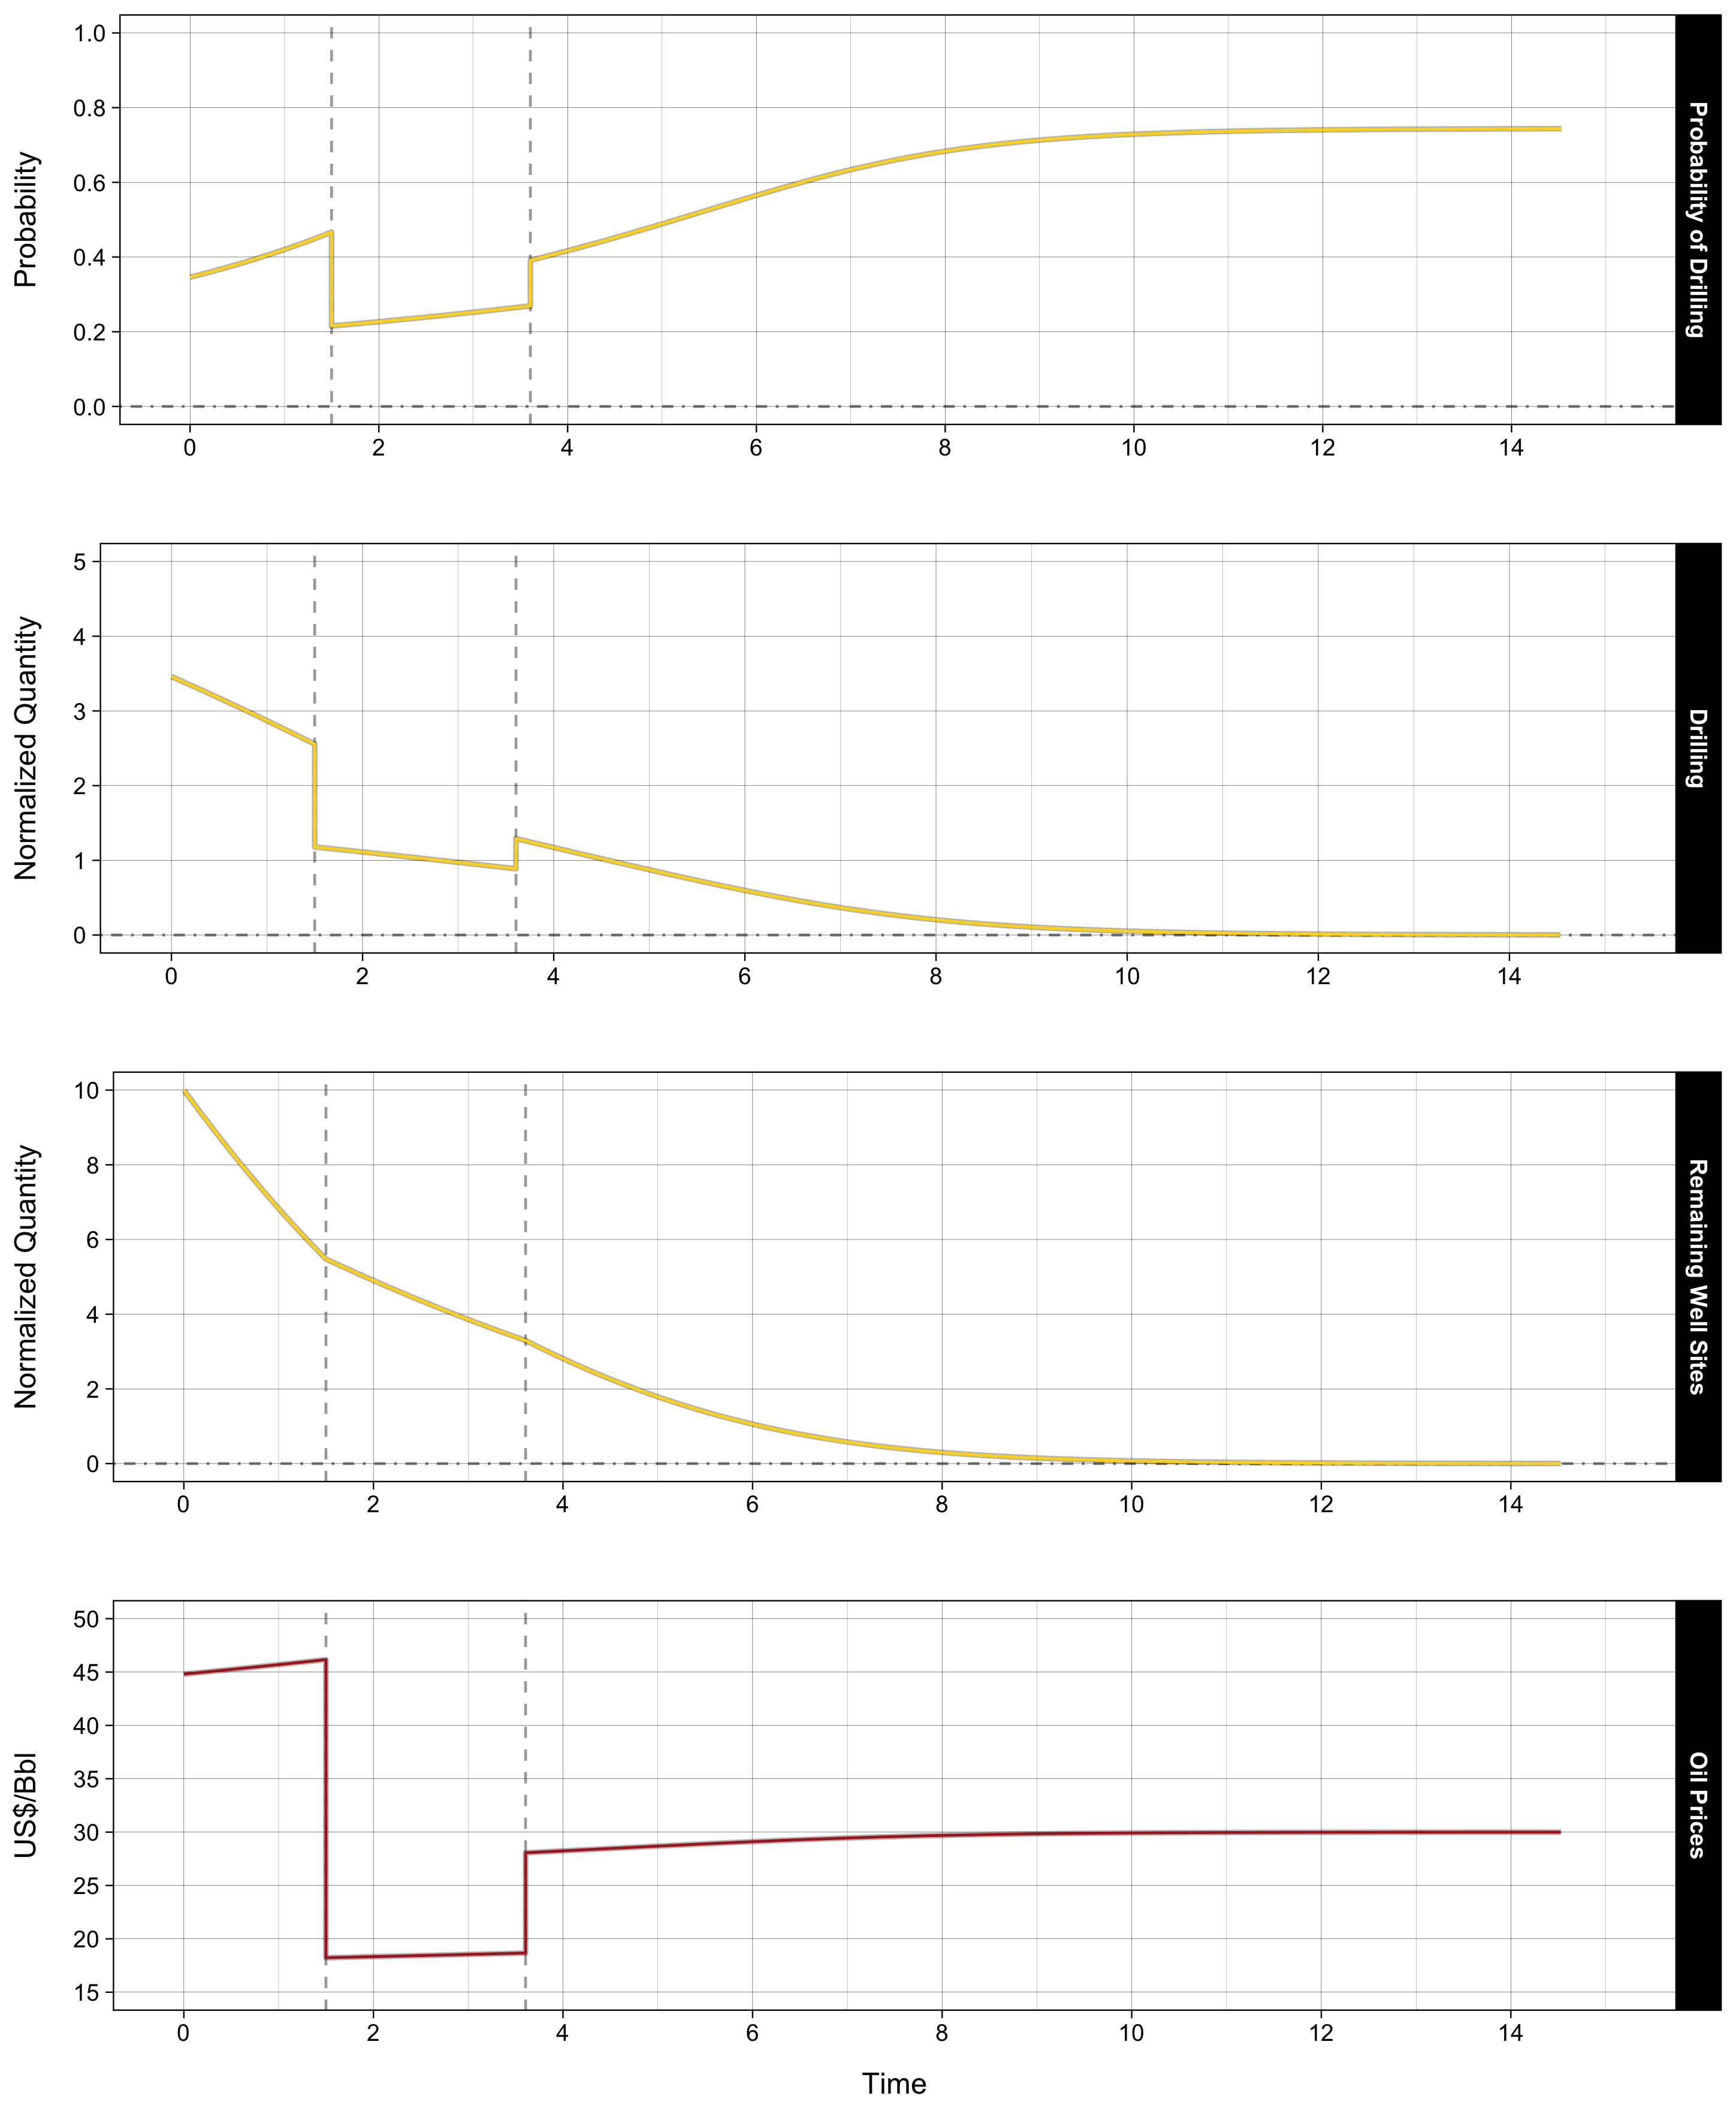
\includegraphics[scale = 0.15]{04_Chapter-3/00A_Figures/Figure_Equlibrium-Paths_Endogenous-Price.png}
        \caption{Equilibrium Paths under Unexpected Demand Shocks}
        \caption*{
            {\small
            \textit{Note}: 
            This figure shows the equilibrium paths of drilling probability, drilling, and the measure of well sites, which are obtained from a simulation for two unanticipated demand shocks. For these simulation results, we assume the identical parameter values and cost function utilized to draw the phase diagrams in Figure \ref{Figure:Phase-Diagram_Saddle-Point}.
        }}
        \label{Figure:Equilibrium-Paths-under-Unexpected-Demand-Shocks}
    \end{figure}
}
